There are some operations on real numbers that either preserve or reverse the relationship between any two real numbers (or some meaningful subset of the real line).

\underline{Rules for Inequalities}

These following operations are order \emph{preserving.} Note that, for each of these, the same relationship is true when one replaces each instance of \(<\) with any one of \(>, \le, \ge.\)

\begin{enumerate}
    \item For any real number, \(c,\) if \(a < b\) then \(a + c < b + c.\) 
    \item For any positive real number, \(c>0,\) if \(a < b\) then \(ac < bc.\)
    \item For any positive real number, \(c>0,\) if \(0< a < b\) then \(a^c < b^c.\)
\end{enumerate}

\desmos{c1g1tvbhqg}{100}{600}

A number line displaying the relationship between \(a,\) \(b,\) \(a+c,\) and \(b+c\)

\desmos{gaog8zcdxq}{100}{600}

A number line dispalying the relationship between \(a,\) \(b,\) \(ac,\) and \(bc.\)

\desmos{ntx79bxwse}{100}{600}
\begin{image}
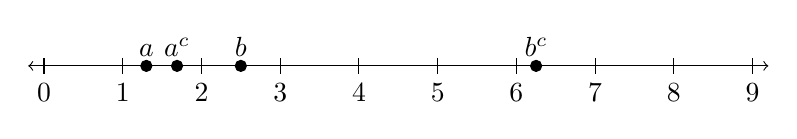
\begin{tikzpicture}
    \draw[<->] (-0.2, 0) -- (9.2, 0);

    \foreach \x in {0, 1, 2, 3, 4, 5, 6, 7, 8, 9} {
        \draw (\x, -0.1) -- (\x, 0.1);
        \node[below] at (\x, -0.1) {$\x$};
    }
    \filldraw[black] (1.3, 0) circle (2pt) node[above]{$a$};
    \filldraw[black] (2.5, 0) circle (2pt) node[above]{$b$};
    \filldraw[black] (6.25, 0) circle (2pt) node[above]{$b^c$};
    \filldraw[black] (1.69, 0) circle (2pt) node[above]{$a^c$};

    \end{tikzpicture}
\end{image}

A number line displaying the relationship between \(a,\) \(b,\) \(a^c,\) and \(b^c.\)

The following operations are order \emph{reversing.} Note that each of these are order reversing for any one of our inequalities and that when considering \(\le\) or \(\ge\) the relationships with \(0\) must remain strict inequalities. (i.e. \(<\) or \(>\))

\begin{enumerate}
    \item If \(0<a<b\) then \(\frac{1}{a} > \frac{1}{b}.\)
    \item If \(a<b<0\) then \(\frac{1}{a} > \frac{1}{b}.\)
    \item For any negative real number, \(c<0,\) if \(a<b,\) then \(ac > bc.\)
\end{enumerate}

Note that any of the above statements can be ``reversed.'' For example it is also true that for any positive real number, \(c>0,\) if \(0< a^c < b^c\) then \(a < b.\) The following questions are perhaps best solved by applying the reverse direction of these rules.